\documentclass[a4paper]{article}
\usepackage[top=1in, bottom=1.25in, left=1.25in, right=1.25in]{geometry}
\usepackage{amsmath}
\usepackage{multicol}
\usepackage{graphicx}
\usepackage[utf8]{inputenc}
\usepackage[english]{babel}
\setlength{\parskip}{0.03cm plus4mm minus3mm}
\RequirePackage{ltxcmds}[2010/12/07]
\usepackage{array}
\usepackage{hyperref}
\renewcommand{\arraystretch}{1.5}
%\setlength{\arrayrulewidth}{1mm}
%opening
\title{Homodyne receiver}

\begin{document}

\maketitle

\clearpage

\section{Homodyne receiver}

This block of code simulates the reception and demodulation of an optical signal (which is the input signal of the system) outputing a binary signal. A simplified schematic representation of this block is shown in figure \ref{MQAM_receiver_block_diagram_simple}.

\begin{figure}[h]
	\centering
	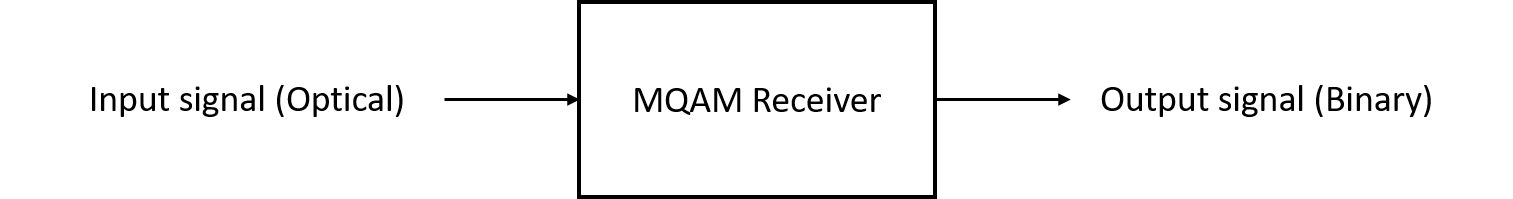
\includegraphics[width=0.8\textwidth]{../lib/homodyne_receiver/figures/MQAM_receiver_block_diagram_simple}
	\caption{Basic configuration of the MQAM receiver}\label{MQAM_receiver_block_diagram_simple}
\end{figure}

\subsection*{Functional description}

This block accepts one optical input signal and outputs one binary signal that corresponds to the M-QAM demodulation of the input signal. It is a complex block (as it can be seen from figure \ref{MQAM_receiver_block_diagram}) of code made up of several simpler blocks whose description can be found in the \textit{lib} repository.

In can also be seen from figure \ref{MQAM_receiver_block_diagram} that there's an extra internal (generated inside the homodyne receiver block) input signal generated by the \textit{Clock}. This block is used to provide the sampling frequency to the \textit{Sampler}.


\begin{figure}[h]
	\centering
	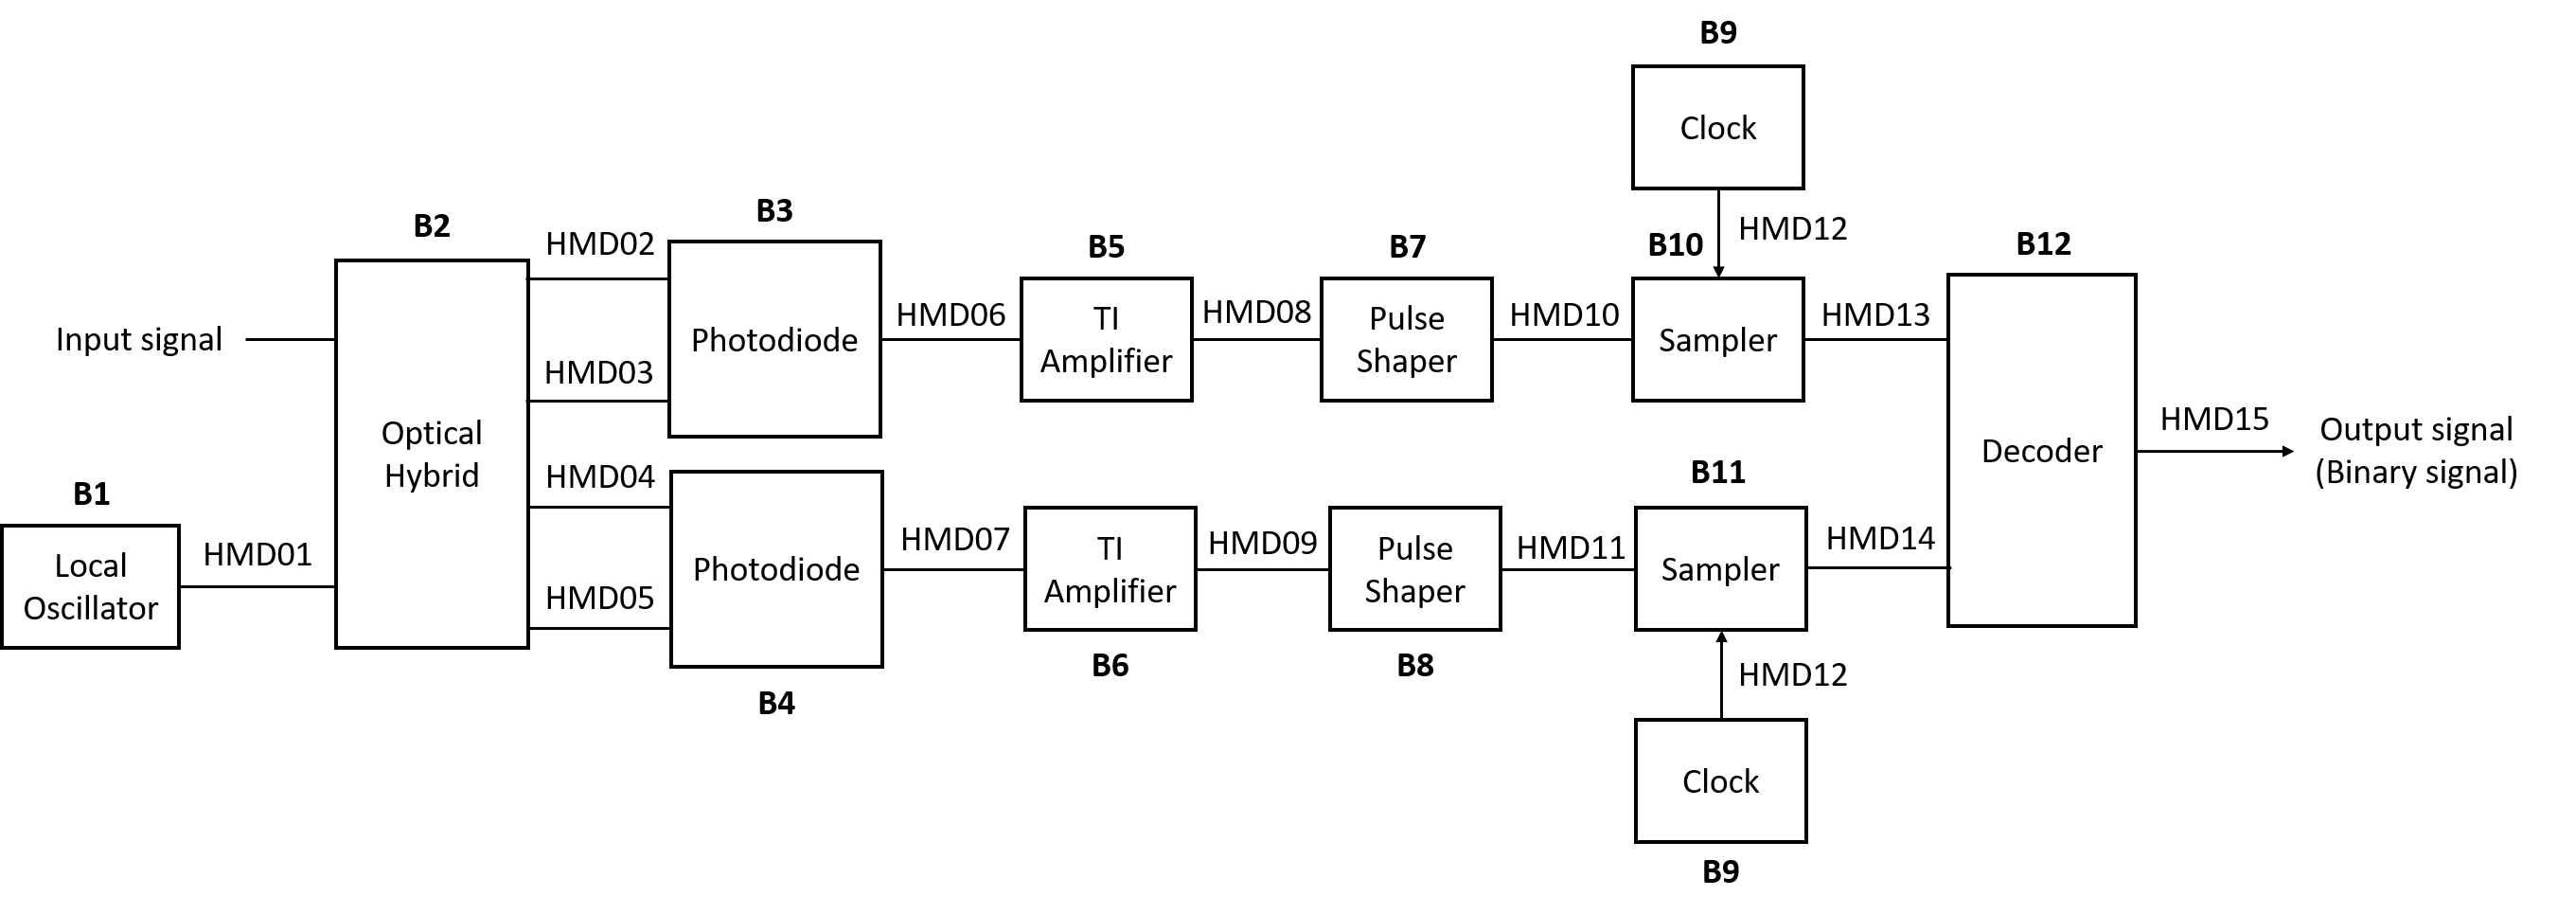
\includegraphics[width=\textwidth]{../lib/homodyne_receiver/figures/MQAM_receiver_block_diagram}
	\caption{Schematic representation of the block homodyne receiver.}\label{MQAM_receiver_block_diagram}
\end{figure}

\subsection*{Input parameters}

This block has some input parameters that can be manipulated by the user in order oto change the basic configuration of the receiver. Each parameter has associated a function that allows for its change. In the following table (table~\ref{table}) the input parameters and corresponding functions are summarized.

\begin{table}[h]
	\begin{center}
		\begin{tabular}{| m{3,5cm} | m{5,8cm} |  m{2,5cm} | m{4cm} | }
			\hline
			\textbf{Input parameters} & \textbf{Function} & Type & \textbf{Accepted values} \\ \hline
			IQ amplitudes & setIqAmplitudes & Vector of coordinate points in the I-Q plane & \textbf{Example} for a 4-qam mapping: \{ \{ 1.0, 1.0 \}, \{ -1.0, 1.0 \}, \{ -1.0, -1.0 \}, \{ 1.0, -1.0 \} \} \\ \hline
			Local oscillator power (in dBm) & setLocalOscillatorOpticalPower\_dBm & double(t\_real) & Any double greater than zero\\ \hline
			Local oscillator phase & setLocalOscillatorPhase & double(t\_real) & Any double greater than zero\\ \hline
			Responsivity of the photodiodes & setResponsivity & double(t\_real) &$\in$ [0,1] \\ \hline
			Amplification (of the TI amplifier) & setAmplification & double(t\_real) & Positive real number\\ \hline
			Noise amplitude (introduced by the TI amplifier) & setNoiseAmplitude & double(t\_real) & Real number greater than zero \\ \hline
			Samples to skipe & setSamplesToSkip & int(t\_integer) &  \\ \hline
			Save internal signals & setSaveInternalSignals & bool & True or False\\ \hline
			Sampling period & setSamplingPeriod & double & Givem by \textit{symbolPeriod}/\textit{samplesPerSymbol}\\
			\hline
		\end{tabular}
		\caption{List of input parameters of the block MQAM receiver} \label{table}
	\end{center}
\end{table}

\pagebreak

\subsection*{Methods}

HomodyneReceiver(vector$<$Signal *$>$ \&inputSignal, vector$<$Signal *$>$ \&outputSignal) (\textbf{constructor})
\bigbreak
void setIqAmplitudes(vector$<$t\_iqValues$>$ iqAmplitudesValues)
\bigbreak
vector$<$t\_iqValues$>$ const getIqAmplitudes(void)
\bigbreak
void setLocalOscillatorSamplingPeriod(double sPeriod)
\bigbreak
void setLocalOscillatorOpticalPower(double opticalPower)
\bigbreak
void setLocalOscillatorOpticalPower\_dBm(double opticalPower\_dBm)
\bigbreak
void setLocalOscillatorPhase(double lOscillatorPhase)
\bigbreak
void setLocalOscillatorOpticalWavelength(double lOscillatorWavelength)
\bigbreak
void setSamplingPeriod(double sPeriod)
\bigbreak
void  setResponsivity(t\_real Responsivity)
\bigbreak
void setAmplification(t\_real Amplification)
\bigbreak
void setNoiseAmplitude(t\_real NoiseAmplitude)
\bigbreak
void setImpulseResponseTimeLength(int impResponseTimeLength)
\bigbreak
void setFilterType(PulseShaperFilter fType)
\bigbreak
void setRollOffFactor(double rOffFactor)
\bigbreak
void setClockPeriod(double per)
\bigbreak
void setSamplesToSkip(int sToSkip)

\pagebreak

\subsection*{Input Signals}

\subparagraph*{Number:} 1

\subparagraph*{Type:} Optical signal

\subsection*{Output Signals}

\subparagraph*{Number:} 1

\subparagraph*{Type:} Binary signal

\subsection*{Example}

\subsection*{Sugestions for future improvement}

\clearpage

\section{Local Oscillator}

This block simulates a local oscillator which can have shot noise or not. It produces one output complex signal and it doesn't accept input signals.

\subsection*{Input Parameters}

\begin{itemize}
	\item opticalPower\{ 1e-3 \}
	\item wavelength\{ 1550e-9 \}
	\item frequency\{ SPEED\_OF\_LIGHT / wavelength \}
	\item phase\{ 0 \}
	\item samplingPeriod\{ 0.0 \}
	\item shotNoise\{ false \}
\end{itemize}

\subsection*{Methods}

LocalOscillator() {}
\bigbreak
LocalOscillator(vector$<$Signal *$>$ \&InputSig, vector$<$Signal *$>$ \&OutputSig) :Block(InputSig, OutputSig)\{\};
\bigbreak
void initialize(void);
\bigbreak
bool runBlock(void);
\bigbreak
void setSamplingPeriod(double sPeriod);
\bigbreak
void setOpticalPower(double oPower);
\bigbreak
void setOpticalPower\_dBm(double oPower\_dBm);
\bigbreak
void setWavelength(double wlength);
\bigbreak
void setPhase(double lOscillatorPhase);
\bigbreak
void setShotNoise(bool sNoise);

\subsection*{Functional description}

This block generates a complex signal with a specified phase given by the input parameter \textit{phase}.

It can have shot noise or not which corresponds to setting the \textit{shotNoise} parameter to True or False, respectively. If there isn't shot noise the the output of this block is given by $0.5*\sqrt{OpticalPower}*ComplexSignal$. If there's shot noise then a random gaussian distributed noise component is added to the \textit{OpticalPower}.

\pagebreak
\subsection*{Input Signals}

\subparagraph*{Number:} 0

\subsection*{Output Signals}

\subparagraph*{Number:} 1

\subparagraph*{Type:} Optical signal

\subsection*{Examples}

\subsection*{Sugestions for future improvement}



\clearpage

\section{Optical hybrid}

This block simulates an optical hybrid. It accepts two input signals corresponding to the signal and to the local oscillator. It generates four output complex signals separated by $90^\circ$ in the complex plane. Figure ~\ref{opticalhybrid} shows a schematic representation of this block.

\begin{figure}[h]
	\centering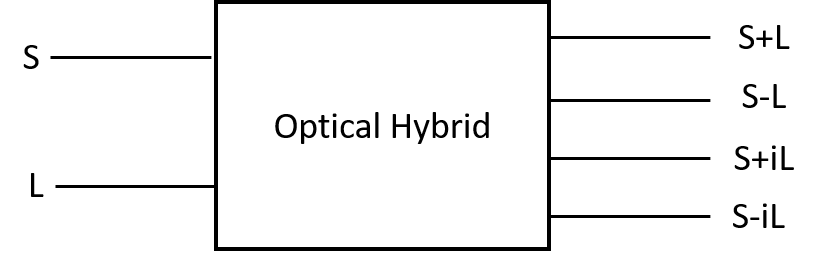
\includegraphics[width=0.6\textwidth]{../homodyne_receiver/figures/optical_hybrid.png}
	\caption{Schematic representation of an optical hybrid}\label{opticalhybrid}
\end{figure}

\subsection*{Input Parameters}

\begin{itemize}
	\item outputOpticalPower\{ 1e-3 \} 
	\item outputOpticalWavelength\{ 1550e-9 \}
	\item outputOpticalFrequency\{ SPEED\_OF\_LIGHT / wavelength \}
	\item powerFactor\{0.5\}
\end{itemize}

\subsection*{Methods}
 
OpticalHybrid() {}
\bigbreak
OpticalHybrid(vector$<$Signal *$>$ \&InputSig, vector$<$Signal *$>$ \&OutputSig) :Block(InputSig, OutputSig) {}
\bigbreak
void initialize(void)
\bigbreak
bool runBlock(void)
\bigbreak
void setOutputOpticalPower(double outOpticalPower)
\bigbreak
void setOutputOpticalPower\_dBm(double outOpticalPower\_dBm)
\bigbreak
void setOutputOpticalWavelength(double outOpticalWavelength)
\bigbreak
void setOutputOpticalFrequency(double outOpticalFrequency) 
\bigbreak
void setPowerFactor(double pFactor)

\subsection*{Functional description}

This block accepts two  input signals corresponding to the signal to be demodulated ($S$) and to the local oscillator ($L$). It generates four output optical signals given by $\textit{powerFactor}\times(S+L)$, $\textit{powerFactor}\times(S-L)$,$\textit{powerFactor}\times(S+iL)$, $\textit{powerFactor}\times(S-iL)$. The input parameter \textit{powerFactor} assures the conservation of optical power.

\pagebreak

\subsection*{Input Signals}

\subparagraph*{Number:} 2

\subparagraph*{Type:} Optical (OpticalSignal)

\subsection*{Output Signals}

\subparagraph*{Number:} 4

\subparagraph*{Type:} Optical (OpticalSignal)

\subsection*{Examples} 

\begin{figure}[h]
	\centering
	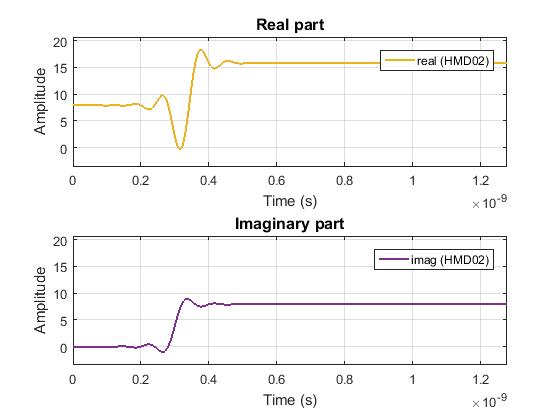
\includegraphics[width=\textwidth]{../homodyne_receiver/figures/OpticalHybrid_output}
	\caption{Example of one of the output signals of this block for a binary sequence 01}\label{OpticalHybrid_output}
\end{figure}

\subsection*{Sugestions for future improvement}

\documentclass[../../sdf/tex/BPSK_system.tex]{subfiles}
\graphicspath{{../../images/}}
%opening
\onlyinsubfile{\title{Photodiode}}
\date{}

\begin{document}

\onlyinsubfile{\maketitle}

\subsection*{Input Parameters}

\begin{multicols}{2}
	\begin{itemize}
		\item setResponsivity
		\item useNoise
	\end{itemize}
\end{multicols}

\subsection*{Functional Description}

This block accepts two complex signals and outputs one real signal built from an evaluation of the power of the input signals and their subsequent subtraction. The responsivity is defined by the value of \textit{Responsivity}. This block also adds random gaussian distributed shot noise with an amplitude defined by the power of the inputs. The shot noise is activated by the boolean variable set by the \textit{useNoise} parameter.

\subsection*{Input Signals}

\textbf{Number}: 2

\textbf{Type}: Complex signal (ContinuousTimeContinuousAmplitude)

\subsection*{Output Signals}

\textbf{Number}: 1

\textbf{Type}: Real signal (ContinuousTimeContinuousAmplitude)

\end{document}
\clearpage

\section{TI Amplifier}

\maketitle

This block has one input signal and one output signal both corresponding to electrical signals. The output signal corresponds to the amplification of the input signal with added noise.


\subsection*{Input Parameters}

\begin{itemize}
	\item amplification\{1e6\}
	\item noiseamp\{ 1e-4 \}
\end{itemize}

\subsection*{Methods}
 
TIAmplifier() {}
\bigbreak
TIAmplifier(vector$<$Signal *$>$ \&InputSig, vector$<$Signal *$>$ \&OutputSig) :Block(InputSig, OutputSig) {}
\bigbreak
void initialize(void)
\bigbreak
bool runBlock(void)
\bigbreak
void setAmpplification(\texttt{t\_real} Amplification)
\bigbreak
void setNoiseAmpplitude(\texttt{t\_real} NoiseAmplitude)

\subsection*{Functional description}

The output signal is the product of the input signal with the parameter \textit{amplification} plus a component that corresponds to the noise introduced by the amplification of the signal. 

\pagebreak

\subsection*{Input Signals}

\subparagraph*{Number:} 1

\subparagraph*{Type:} Electrical (TimeContinuousAmplitudeContinuousReal)

\subsection*{Output Signals}

\subparagraph*{Number:} 1

\subparagraph*{Type:} Electrical (TimeContinuousAmplitudeContinuousReal)

\subsection*{Examples} 

\begin{figure}[h]
	\centering
	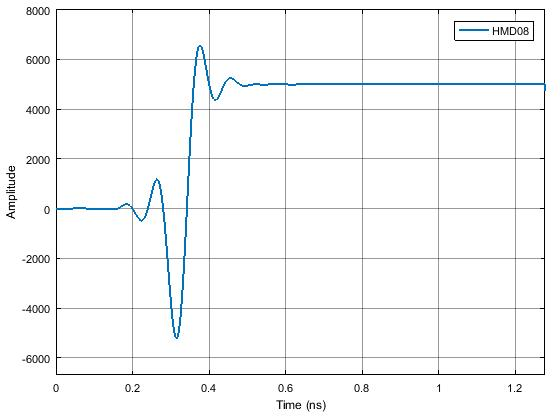
\includegraphics[width=\textwidth]{../homodyne_receiver/figures/TIAmplifier_output}
	\caption{Example of the output signal of the amplifier block for a binary sequence 01. Note the scale of the y axis in comparison to the one in the output signal of the photodiode. The shape of the signal is the same as expected}\label{TIAmplifier_output}
\end{figure}

\subsection*{Sugestions for future improvement}


\clearpage

\section{Pulse shaper}

This block applies an electrical filter to the signal. It accepts one input signal that is a sequence of Dirac delta functions and it produces one output signal continuous in time and in amplitude.

\subsection*{Input Parameters}

\begin{itemize}
	\item filterType\{RaisedCosine\} \linebreak
	\item impulseResponseTimeLength\{16\}\linebreak (int) 
	\linebreak (This parameter is given in units of symbol period)
	\item rollOfFactor\{0.9\} \linebreak
	(real $\in$ [0,1])
\end{itemize}

\subsection*{Methods}

PulseShaper(vector$<$Signal *$>$ \&InputSig, vector$<$Signal *$>$ OutputSig) :FIR$\_$Filter(InputSig, OutputSig)\{\};
\bigbreak	
void initialize(void);
\bigbreak	
void setImpulseResponseTimeLength(int impResponseTimeLength)
\bigbreak
int const getImpulseResponseTimeLength(void)
\bigbreak	
void setFilterType(PulseShaperFilter fType)
\bigbreak
PulseShaperFilter const getFilterType(void)
\bigbreak	
void setRollOffFactor(double rOffFactor)
\bigbreak
double const getRollOffFactor()

\subsection*{Functional Description}

The type of filter applied to the signal can be selected trough the input parameter \textit{filterType}. Currently the only available filter is a raised cosine.

The filter's transfer function is defined by the vector \textit{impulseResponse}. The parameter \textit{rollOfFactor} is a characteristic of the filter and is used to define its transfer function.

\subsection*{Input Signals}

\subparagraph*{Number}: 1

\subparagraph*{Type}: Sequence of Dirac Delta functions (ContinuousTimeDiscreteAmplitude)

\subsection*{Output Signals}

\subparagraph*{Number}: 1

\subparagraph*{Type}: Sequence of impulses modulated by the filter (ContinuousTimeContinuousAmplitude)

\subsection*{Example}

\begin{figure}[h]
	\centering
	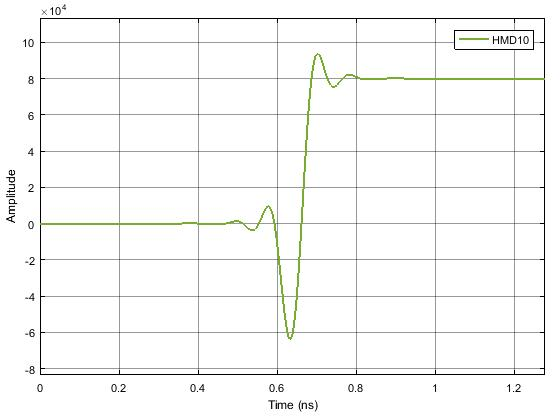
\includegraphics[width=\textwidth]{../homodyne_receiver/figures/PulseShaper_output}
	\label{MQAM6_DeterministicAppendZeros}\caption{Example of a signal generated by this block for the initial binary signal 0100...}
\end{figure}

\subsection*{Sugestions for future improvement}

Include other types of filters.

\clearpage

\section{Sampler}

\maketitle

This block can work in two configurations: with an external clock or without it. In the latter it accepts two input signals one being the clock and the other the signal to be demodulated. In the other configuration there's only one input signal which is the signal. 

The output signal is obtained by sampling the input signal with a predetermined samplig rate provided either internally or by the clock.

\subsection*{Input Parameters}

\begin{itemize}
	\item samplesToSkip\{ 0 \}
\end{itemize}

\subsection*{Methods}
 
Sampler() {}
\bigbreak
Sampler(vector$<$Signal *$>$ \&InputSig, vector$<$Signal *$>$ \&OutputSig) :Block(InputSig, OutputSig) {}
\bigbreak
void initialize(void)
\bigbreak
bool runBlock(void)
\bigbreak
void setSamplesToSkip(\texttt{t\_integer} sToSkip)

\subsection*{Functional description}

This block can work with an external clock or without it. 

In the case of having an external clock it accepts two input signals. The signal to be demodulate which is complex and a clock signal that is a sequence of Dirac delta functions with a predetermined period that corresponds to the sampling period. The signal and the clock signal are scanned and when the clock has the value of 1.0 the correspondent complex value of the signal is placed in the buffer corresponding to the output signal.

There's a detail worth noting. The electrical filter has an impulse response time length of 16 (in units of symbol period). This means that when modulating a bit the spike in the signal corresponding to that bit will appear 8 units of symbol period later. For this reason there's the need to skip the earlier samples of the signal when demodulating it. That's the purpose of the \textit{samplesToSkip} parameter.

Between the binary source and the current block the signal is filtered twice which means that this effect has to be taken into account twice. Therefore the parameter \textit{samplesToSkip} is given by $2*8*samplesPerSymbol$. 




\pagebreak

\subsection*{Input Signals}

\subparagraph*{Number:} 1

\subparagraph*{Type:} Electrical real (TimeContinuousAmplitudeContinuousReal)

\subsection*{Output Signals}

\subparagraph*{Number:} 1

\subparagraph*{Type:} Electrical real (TimeDiscreteAmplitudeContinuousReal)

\subsection*{Examples} 

\begin{figure}[h]
	\centering
	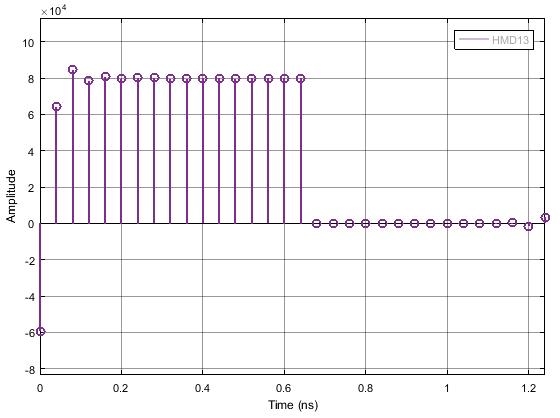
\includegraphics[width=\textwidth]{../homodyne_receiver/figures/Sampler_output}
	\caption{Example of the output signal of the sampler}\label{Sampler_output}
\end{figure}

\subsection*{Sugestions for future improvement}

\clearpage

\section{Clock}

This block doesn't accept any input signal. It outputs one signal that corresponds to a sequence of Dirac's delta functions with a user defined \textit{period}.

\subsection*{Input Parameters}

\begin{itemize}
	\item period\{ 0.0 \};
	\item samplingPeriod\{ 0.0 \};
\end{itemize}

\subsection*{Methods}

Clock() {}
\bigbreak
Clock(vector$<$Signal *$>$ \&InputSig, vector$<$Signal *$>$ \&OutputSig) :Block(InputSig, OutputSig) {}
\bigbreak
void initialize(void)
\bigbreak
bool runBlock(void)
\bigbreak
void setClockPeriod(double per)
\bigbreak
void setSamplingPeriod(double sPeriod)

\subsection*{Functional description}


\pagebreak

\subsection*{Input Signals}

\subparagraph*{Number:} 0

\subsection*{Output Signals}

\subparagraph*{Number:} 1

\subparagraph*{Type:} Sequence of Dirac's delta functions. (TimeContinuousAmplitudeContinuousReal)

\subsection*{Examples}

\begin{figure}[h]
	\centering
	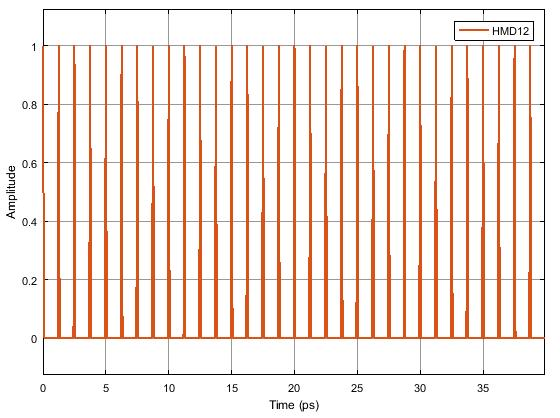
\includegraphics[width=\textwidth]{./lib/clock/figures/Clock_output}
	\caption{Example of the output signal of the clock}\label{Clock_output}
\end{figure}

\subsection*{Sugestions for future improvement}


\clearpage

\section{Decoder}

This block accepts a complex electrical signal and outputs a sequence of binary values (0's and 1's). Each point of the input signal corresponds to a pair of bits.

\subsection*{Input Parameters}

\begin{itemize}
	\item\texttt{t\_integer} m\{ 4 \}
	\item vector$<$\texttt{t\_complex}$>$ iqAmplitudes\{ \{ 1.0, 1.0 \},\{ -1.0, 1.0 \},\{ -1.0, -1.0 \},\{ 1.0, -1.0 \} \};
\end{itemize}

\subsection*{Methods}

Decoder() {}
\bigbreak
Decoder(vector$<$Signal *$>$ \&InputSig, vector$<$Signal *$>$ \&OutputSig) :Block(InputSig, OutputSig) {}
\bigbreak
void initialize(void)
\bigbreak
bool runBlock(void)
\bigbreak
void setM(int mValue)
\bigbreak
void getM()
\bigbreak
void setIqAmplitudes(vector$<$\texttt{t\_iqValues}$>$ iqAmplitudesValues)
\bigbreak
vector$<$\texttt{t\_iqValues}$>$getIqAmplitudes()

\subsection*{Functional description}

This block makes the correspondence between a complex electrical signal and pair of binary values using a predetermined constellation.

To do so it computes the distance in the complex plane between each value of the input signal and each value of the \textit{iqAmplitudes} vector selecting only the shortest one. It then converts the point in the IQ plane to a pair of bits making the correspondence between the input signal and a pair of bits.

\pagebreak

\subsection*{Input Signals}

\subparagraph*{Number:} 1

\subparagraph*{Type:} Electrical complex (TimeContinuousAmplitudeContinuousReal)

\subsection*{Output Signals}

\subparagraph*{Number:} 1

\subparagraph*{Type:} Binary

\subsection*{Examples}

As an example take an input signal with positive real and imaginary parts. It would correspond to the first point of the \textit{iqAmplitudes} vector and therefore it would be associated to the  pair of bits $00$.

\begin{figure}[h]
	\centering
	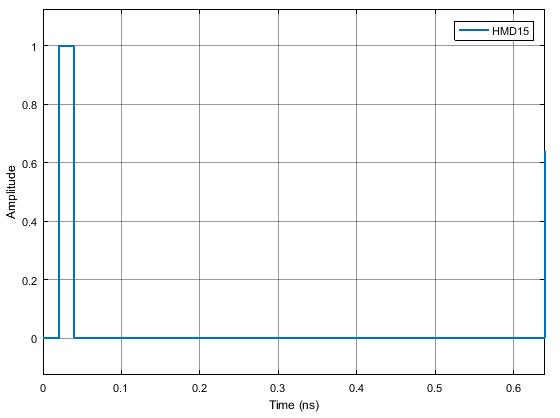
\includegraphics[width=\textwidth]{./lib/decoder/figures/Decoder_output}
	\caption{Example of the output signal of the decoder for a binary sequence 01. As expected it reproduces the initial bit stream}\label{Decoder_output}
\end{figure}

\subsection*{Sugestions for future improvement}


\end{document} 